\section{Grundlagen}

\subsection{Geschichtlicher Hintergrund}\label{sec:story-background}
% Demokratie
Der geschichtliche Hintergrund von Nachrichten als wichtiges Medium in einer Demokratie reicht zurück bis zu den Anfängen der Demokratie in der Antike\textcolor{red}{[cite?]}.
Eine Demokratie ist einer Form der Regierung, bei der die Macht bei der Bevölkerung liegt.
Zusammenfassen lässt sich diese Form der Regierung durch Thomas Paine und Abraham Lincolns moderne Formel \glqq Regierung des Volkes, durch das Volk, für das Volk\grqq{} \cite{lincoln}.
Dies lässt sich auch erkennen, wenn man sich den Ursprung des Wortes Demokratie anschaut.
Demokratie setzt sich zusammen aus den altgriechischen Wörtern Demos (\textgreek{δῆμος}) für Volk und Kratos (\textgreek{κράτος}) für Herrschaft.
Damit die Bevölkerung jedoch Herrschaft über die Regierung ausüben kann, muss diese über politische Ereignisse und Entscheidungen informiert sein.
Eine unbeeinflusste Berichterstattung ist daher eine Grundvoraussetzung für eine funktionierende Demokratie, weil nur so die Bevölkerung in der Lage ist, eine informierte Entscheidung zu treffen. \\

% Zeitung allgemein
Obwohl der geschichtliche Hintergrund bis in die Antike zurückreicht, ist die moderne Form der Nachrichtenberichterstattung erst in den letzten Jahrhunderten entstanden.
Die \textit{Avisa Relation oder Zeitung}\footnote{Die Zeitung ist ebenfalls unter \textit{Aviso Relation oder Zeitung} auffindbar.} war die erste regelmäßig erscheinende Zeitung in Europa \cite{aviso-relation-oder-zeitung}.
Die erste Ausgabe erschien 1609 und beinhaltete Nachrichten aus verschiedenen Teilen Europas\footnote{Die erste Ausgabe trug den Untertitel: \textit{Was sich begeben vnd zugetragen hat /in Deutsch: vnd Welschland / Spannien / Niederlandt / Engellandt /Franckreich / Vngern / Osterreich / Schweden / Polen / vnnd in allen Provintzen / in Ost: vnnd West-Indien etc.}}.
Diese Nachrichten berichteten über militärische, politische und wirtschaftliche Ereignisse und Relationen zwischen den verschiedenen Staaten.
Aufgrund dieser Inhalte war die Zeitung vor allem für die Oberschicht interessant.
Diese Oberschicht bestand aus Adeligen, Diplomaten, Kaufleuten und Gelehrten.
Bis zum Ende des 18. Jahrhundert waren die meisten Zeitungen nicht für die breite Masse der Bevölkerung gedacht, sondern für eine kleine, privilegierte Gruppe.
Zu Beginn des 19. Jahrhunderts begann der Aufstieg des radikalen Journalismus, welcher sich gegen die bestehende aristokratische Ordnung richtete \cite{media-democracy}.
Erst mit der Penny Press in den 1830ern wurde die Zeitung für die breite Masse tauglich \cite{precursor-media-penny-press}.
Das lag daran, dass der Inhalt dieser Zeitungen sich nun auch an Arbeiter und Immigranten richtete.
Die Penny Press war für ihren Sensationsjournalismus bekannt und berichtete über Kriminalfälle und Skandale \cite{penny-press}.\\

% Lippmann
Mit der Zeit entwickelten sich Zeitungen von einem Medium für die Oberschicht zu einem Medium für die breite Masse.
Ebenfalls wurde dadurch die Relevanz von Zeitungen für die Demokratie immer größer.
Wie bereits erwähnt, ist eine unbeeinflusste Berichterstattung eine Grundvoraussetzung für eine funktionierende Demokratie.
Diese Grundvoraussetzung wurde nach dem Ende des Ersten Weltkriegs erschüttert.
Der Journalist Walter Lippmann schrieb 1920 in seinem Buch \textit{Liberty and the News} über Propaganda und die Manipulation der Bevölkerung durch die Medien \cite{liberty-and-news}.
Konkret schrieb er:
\begin{quote}
    \glqq Wenn diejenigen, die sie kontrollieren, sich das Recht anmaßen, nach ihrem eigenen Gewissen zu bestimmen, was berichtet werden soll und zu welchem Zweck, ist die Demokratie nicht funktionsfähig\grqq{}\footnote{Sinngemäße Übersetzung}.
\end{quote}
1922 machte Lippmann erneut mit seinem Buch \textit{Public Opinion} auf die Gefahr der Manipulation durch die Medien aufmerksam \cite{public-opinion}.
Laut Lippmann muss die Bevölkerung die Fähigkeit besitzen Informationen kritisch zu hinterfragen.
Im Jahre 1925 schreibt Lippmann in seinem Buch \textit{The Phantom Public} darüber, dass die Bevölkerung nicht in der Lage ist sich umfassend mit allen politischen Fragen auseinanderzusetzen \cite{phantom-public}.
Seine Folgerung daraus ist, dass die Bevölkerung auf eine kleine Gruppe von Personen mit Expertise angewiesen ist. \\

% Dewey
Der amerikanische Philosoph John Dewey stimmte der Kritik von Lippmann zu.
Allerdings warnte Dewey vor der Gefahr, dass die Bevölkerung dadurch Informationen nur noch passiv aufnimmt.
Dewey schrieb bereits 1916 in seinem Buch \textit{Democracy and Education} \cite{democracy-and-education}:
\begin{quote}
    \glqq Eine Demokratie ist mehr als eine Regierungsform; sie ist in erster Linie eine Form des Zusammenlebens, der gemeinsamer, kommunizierten Erfahrung\grqq{}\footnote{Sinngemäße Übersetzung}.
\end{quote}
1927 betonte Dewey in seinem Buch \textit{The Public and its Problems}, dass die Bevölkerung aktiv an der politischen Debatte teilnehmen muss \cite{public-problems}.
Im Allgemeinem betont Dewey die Notwendigkeit von Bildung, um eine kritisch hinterfragende und informierte Bevölkerung zu schaffen.
Die Debatte zwischen Lippmann und Dewey war einer der größten Debatten des zwanzigsten Jahrhunderts über die Rolle von Journalismus in einer Demokratie \cite{lippmann-dewey-debate}. \\

\textcolor{red}{TODO: Zwischenfazit (siehe Feedback)}
\textcolor{red}{TODO: Einleitung rechtliche Rahmenbedingungen in Deutschland (siehe Feedback)}

% Deutschland
Speziell in der Bundesrepublik Deutschland wird die Meinungsfreiheit durch das Grundgesetz (§ 5 Abs. 1 GG) geschützt \cite{gg}:
\begin{quote}
    \glqq Jeder hat das Recht, seine Meinung in Wort, Schrift und Bild frei zu äußern und zu verbreiten und sich aus allgemein zugänglichen Quellen ungehindert zu unterrichten.
    Die Pressefreiheit und die Freiheit der Berichterstattung durch Rundfunk und Film werden gewährleistet.
    Eine Zensur findet nicht statt.\grqq{}
\end{quote}
Neben den Printmedien fallen auch Rundfunk und Telemedien in Deutschland unter dieses Gesetz.
Zusätzlich werden diese Medien durch den \ac{RStV} reguliert \cite{rundfunkstaatsvertrag}.
Der \ac{RStV} besagt, dass die öffentlich-rechtlichen Rundfunkanstalten umfassend informieren und die Meinungen der Bevölkerung wiedergeben müssen (§ 11 Abs. 1 \ac{RStV}).
Dieser Absatz macht zusätzlich aufmerksam darauf, dass die demokratischen, sozialen und kulturellen Interessen der Bevölkerung berücksichtigt werden müssen. \\

% Printmedien / Rundfunk / Telemedien
Printmedien und Rundfunk und Telemedien unterscheiden sich in vielerlei Hinsichten.
Während Rundfunk und Telemedien an eine bestimmte Zeit gebunden sind, können Printmedien jederzeit gelesen werden.
Aufgrund der zeitlichen Begrenzung müssen Inhalte sorgfältig kuriert werden.
Durch die lineare Reihenfolge der Inhalte sind bestimmte Inhalte relevanter als andere \cite{rundfunk}.
Aus diesem Grund werden die Nachrichten kurz vor dem Hauptabendprogramm\footnote{Ebenfalls \textit{Prime Time} bezeichnet} platziert.
Die Platzierung richtet sich hierbei an den Lebenszyklus des Publikums.
Der Vorteil im Vergleich zu Printmedien ist, dass Inhalte in Echtzeit veröffentlicht werden können.
Somit können Rundfunk und Telemedien auf aktuelle Ereignisse reagieren\footnote{Beispiele hierfür sind Aufklärung über Verkehrslagen im Rundfunk und sogenannte Breaking News in Telemedien}. \\

% Online-Medien
Aktuell sieht die Situation dank der Digitalisierung und der damit verbundenen Verfügbarkeit von Informationen im Internet anders aus.
Die Bevölkerung ist bei Audio- und Videoinhalten nicht mehr an eine bestimmte Zeit gebunden.
Ebenfalls können Texte und Bilder in Echtzeit veröffentlicht und verbreitet werden.
In vielen Fällen werden die traditionellen Medien ersetzt oder ergänzt.
\textcolor{red}{TODO: Quelle Medienkonsumverhalten (siehe Feedback)}
Durch die einfache Verbreitung von Inhalten kann so ziemlich jede Person mit Internetzugang Journalismus betreiben.
\textcolor{red}{TODO: Journalismus Definition eingrenzen (siehe Feedback)}
Dieser Wandel führt allerdings zu einer Flut an Informationen, welche es schwer macht, relevante Inhalte zu finden.
Ein Weg diese Flut zu bewältigen ist die Nutzung von einem \ac{RS}.
\textcolor{red}{TODO: Übergang weiter ausführen, wieso es RS gibt + vielleicht auch historisch (siehe Feedback)}

\subsection{Recommender system}
% Intro RS
Ein \acf{RS} (zu Deutsch: Empfehlungssystem) ist ein Softwaresystem, welches aus einer gegebenen Menge an Daten eine Teilmenge auswählt, welche für Nutzende relevant ist \cite{recommender-systems}.
\ac{RS} werden in verschiedenen Bereichen eingesetzt.
Beispiel hierfür sind inhaltliche Empfehlungen von Artikeln in Online-Shops oder die Empfehlung von Freunden in sozialen Netzwerken \cite{ecommerce-recommender, social-recommender}.
Ein weiteres Anwendungsgebiet ist die Empfehlung von journalistischen Nachrichten \cite{news-recommender}.
Vorgeschlagene Inhalte von \acp{RS} werden von vielen Personen der Bevölkerung journalistisch kurierten Empfehlungen vorgezogen \cite{recommender-preference, theory-of-machine}.
\textcolor{red}{TODO: Gründe nennen, wieso RS vorgezogen wird (siehe Feedback)}
Da Menschen verschiedene Vorlieben und Interessen besitzen erscheint es logisch, dass Empfehlungen auf individueller Ebene präferiert werden.
Es existieren zahlreiche Möglichkeiten, um ein \ac{RS} zu implementieren.
Primär geht es jedoch darum die Relevanz von Inhalten für Nutzende zu bestimmen und diese zu maximieren. \\

% Überleitung Helberger
Wie bereits im vorherigen \autoref{sec:story-background} erwähnt werden Medien historisch als zentrale Informationsquelle in einem demokratischen System verwendet.
Bezogen auf das Internet kann eine Unterscheidung zwischen verteilter und demokratischer Macht\footnote{Das altgriechische Wort Kratos (\textgreek{κράτος}) kann ebenfalls als Macht übersetzt werden} vorgenommen werden \cite{free-speech-algorithmic}.
\textcolor{red}{TODO: verteilte und demokratische Macht näher ausführen? (siehe Feedback)}
Der Unterschied liegt darin, dass bei der verteilten Macht viele Menschen betroffen werden und eine demokratische Macht viele Menschen mitentscheiden lässt.
Die Rechtswissenschaftlerin und Professorin Natali Helberger beschreibt in ihrem Paper die konkrete Beziehung zwischen \acp{RS} und diesem demokratischen System \cite{democratic-role}.
Medien spielen dabei zwei zentrale Rollen: Sie informieren und schaffen ein vielfältiges öffentliches Forum für einen Meinungsaustausch.
Dies geht Hand in Hand mit der bereits beschriebenen Notwendigkeit zu informieren und der von Dewey beschriebenen Notwendigkeit, dass die Bevölkerung aktiv an der politischen Debatte teilnimmt.
Zum Informieren werden \acp{RS} verwendet.
Dabei kann speziell bei News-\acp{RS} zwischen vier verschiedenen Algorithmen unterschieden werden (content-based, collaborative, knowledge based und hybrid).
Diese Algorithmen werden nachfolgend kurz am Beispiel einer Nachrichtenwebsite vorgestellt.
\textcolor{red}{TODO: Herausstellen: ein Bezug zu Nutzenden? Steht das nicht im Absatz davor? (siehe Feedback)} \\

% Algorithmen
Content-based Filtering empfiehlt ähnliche Inhalte basierend auf Eigenschaften der Inhalte \cite{content-based-rs}.
Die Eigenschaften können beispielsweise Thema, Autor oder Zeitpunkt der Veröffentlichung sein.
In Bezug auf das Beispiel einer Nachrichtenwebsite gibt es eine Person, welche häufig Artikel über Technologie liest.
In diesem Fall würde der Algorithmus weitere Artikel zum Thema Technologie empfehlen.
Collaborative Filtering empfiehlt ähnliche Inhalte basierend auf den Interessen von anderen Nutzenden \cite{collaborative-filtering-rs}.
Um die Interessen von Nutzenden zu ermitteln, muss zunächst Feedback von Nutzenden gesammelt werden.
Dieses Feedback kann explizit oder implizit gesammelt werden.
Beispiel für explizites Feedback ist das Bewerten eines Artikels.
Beispiel für implizites Feedback ist das Klicken auf einen Artikel.
Bezogen auf die Nachrichtenwebsite empfiehlt der Algorithmus Artikeln von Nutzenden mit ähnlichen Interessen, welche positiv bewertet oder häufig geklickt wurden.
Knowledge based Filtering empfiehlt ähnliche Inhalte basierend auf explizitem Wissen über Inhalte \cite{knowledge-based-rs}.
Beim Beispiel der Nachrichtenwebsite würde der Algorithmus Artikel empfehlen, welche sich auf dasselbe Thema beziehen oder von derselben Quelle stammen.
Es ist ebenfalls möglich mehrere der oben genannten Algorithmen zu kombinieren.
Die somit entstehende Kombination wird als ein hybrides \ac{RS} bezeichnet.
Die Kombination aus content-based und collaborative Filtering könnte somit Inhalte empfehlen, welche ähnliche Eigenschaften besitzen und von anderen Nutzenden mit ähnlichen Interessen positiv bewertet wurden.\\

% Formen der Demokratie
Helberger beschreibt ferner drei unterschiedliche Theorien der Demokratie (liberal, partizipativ und deliberativ).
Der Grund dafür ist, dass unterschiedliche Theorien unterschiedliche Anforderungen an die Medien stellen.
Die von Helberger ausgewählten Theorien sind die drei häufigsten untersuchten Theorien in den Medien- und Kommunikationswissenschaften \cite{democratic-theories}.
Zusätzlich werden die drei Theorien in Bezug auf potenzielle \ac{RS} gesetzt.
Für ein besseres Verständnis werden diese Theorien nachfolgend kurz vorgestellt.\\

% Democracy Models
Das liberale Modell der Demokratie stellt die Freiheit der Bevölkerung in den Vordergrund.
Die Bevölkerung soll die Freiheit haben, sich selbst zu informieren.
Dies umfasst auch das Recht, zu entscheiden, welche Informationen mit anderen geteilt werden und somit das Recht auf Privatsphäre.
Ähnlich wie bei der freien Marktwirtschaft wird das liberale Modell von der Annahme getragen, dass die freie Wahl und das Wettbewerbsprinzip förderlich ist.
Dieses Konzept wird metaphorisch als \glqq Marktplatz der Ideen\grqq{} bezeichnet \cite{marketplace-ideas}.
Das partizipative Modell der Demokratie hingegen stellt die Beteiligung der Bevölkerung an der politischen Debatte in den Vordergrund.
Statt sich, wie beim liberalen Modell, selbst zu informieren, soll die Bevölkerung durch die Medien informiert werden.
Inhalte müssen divers genug sein, dass sie alle signifikant relevanten Perspektiven abdecken.
Die Tendenz dieses Modells entfernt sich vom Egoismus hin zum Altruismus. \textcolor{red}{TODO: rework Altruismus (siehe Feedback)}
Ähnlich wie beim partizipativen Modell fokussiert sich das deliberative Modell darauf, dass das Interesse der Bevölkerung über dem eigenen Interesse steht.
Das deliberative Modell besagt jedoch, dass es nicht ausreicht, dass die Bevölkerung nur informiert wird.
Jede Person soll mit konträren Meinungen konfrontiert werden und dazu ermutigt werden sich damit auseinanderzusetzen. \\

% Democracy Models and RS
Die Theorien bzw. Modelle der Demokratie stellen unterschiedliche Anforderungen an die Medien und damit auch an ein \ac{RS}.
Diese Anforderungen können in Konflikt miteinander stehen, weswegen es unmöglich ist, ein \ac{RS} zu entwickeln, welches alle Anforderungen erfüllt.
Gerade die Anforderungen des liberalen und deliberativen Modells stehen besonders in Konflikt miteinander.
Helberger argumentiert, dass es deswegen kein Goldstandard für ein \ac{RS} gibt.
Die Masterarbeit fokussiert sich auf die Anforderungen des liberalen Modells. \textcolor{red}{TODO: Kein liberales Modell (siehe Feedback)}

\subsection{Herausforderungen von Recommender Systems}
% Intro Filterblase
Bezogen auf \acp{RS} stellt die Personalisierung von Inhalten eine Herausforderung für den digitalen Journalismus dar.
Diese Personalisierung von Inhalten sorgt dafür, dass die Diversität von Inhalten und andere Perspektiven eingeschränkt werden \cite{rundfunk}.
Der Effekt wurde von dem Internetaktivisten Eli Pariser im Buch \textit{The Filter Bubble: What the Internet Is Hiding from You} als Filterblase bezeichnet und ist ein bekanntes Problem in der heutigen Gesellschaft \cite{filter-bubble}.
\acp{RS} können zur Erzeugung einer sogenannten Filterblase dazu beitragen, dass Nutzende nur noch Inhalte erhalten, die sie bereits kennen.
Die empfohlenen Inhalte können dann dazu führen, dass Nutzende sich in ihrer eigenen Meinung bestätigt sehen und andere Meinungen weniger oder gar nicht wahrnehmen.
Dieser Effekt wird als Bestätigungsfehler bezeichnet und ist ebenfalls ein bekanntes Problem in der Gesellschaft \cite{reasoning-rule}. \\

% Filterwesen
Informationen werden allerdings nicht erst seit der Einführung von \acp{RS} gefiltert.
Der Mensch ist, wie alle Tiere, ein \glqq Filterwesen\grqq{} und filtert bereits auf natürliche Weise Informationen.
Die visuelle selektive Wahrnehmung ist ein Beispiel dafür \cite{selective-perception}.
Bereits in Rundfunk und Telemedien ist die Entscheidung für einen Sender eine Art Filterung, da Sender unterschiedliche Inhalte anbieten.
Das \ac{RISJ}\footnote{Das \ac{RISJ} ist eine unabhängige Stiftung an der Universität Oxford, welche sich mit Journalismus- und Medienforschung beschäftigt.} konnte in einer Studie zeigen, dass ARD, ZDF und Deutschlandradio von einer politisch linken Mehrheit und RTL und n-tv von einer politisch rechten Mehrheit konsumiert werden \cite{public-service-news}.
Dies kann an den unterschiedlichen Inhalten liegen, welche von den Sendern angeboten werden. \\

% Zurück zu RS
Bei \acp{RS} gibt es ebenfalls die Möglichkeit bewusst unterschiedliche Quellen zu wählen.
Jedoch wird aufgrund des vorliegenden Algorithmus die Diversität der Inhalte mit der Nutzungsdauer immer weiter eingeschränkt.
Wie bereits erwähnt, werden \acp{RS} durch die Verarbeitung von Daten, entweder explizit oder implizit, trainiert.
Vielen Nutzenden ist es jedoch nicht bewusst, dass sie mit der Nutzung von \acp{RS} Daten an die Betreibenden der \acp{RS} weitergeben \cite{privacy-rs}.
Für diesen Fall lassen sich ebenfalls moralische Implikationen für die Gesellschaft ableiten.
Speziell betrifft dies den Wert der Privatsphäre von Einzelpersonen der Bevölkerung.\\

% Privatsphäre
Die verschiedenen Definitionen und Ideen von Privatsphäre wurden 1891 erstmalig als Menschenrecht definiert \cite{history-of-privacy}.
Dort definierten die amerikanischen Juristen Samuel Warren und Louis Brandeis die Privatsphäre als \glqq das Recht in Ruhe gelassen zu werden\grqq{}\footnote{Sinngemäße Übersetzung}.
Eine weitere Definition lässt sich finden im Jahre 1967.
In diesem Jahr veröffentlichte der Professor für öffentliches Recht und Regierung Alan Furman Westin das Buch \textit{Privacy and Freedom} \cite{privacy-and-freedom}.
Dort wird Privatsphäre als \glqq das Recht selbst zu bestimmen, wann, wie und in welchem Umfang Informationen an andere weitergeben werden\grqq{}\footnote{Sinngemäße Übersetzung} definiert.
\acp{RS} funktionieren allerdings nur in Austausch gegen diese Privatsphäre.
Dadurch, dass vielen Nutzenden unbewusst ist, welche und ob Daten weitergeleitet werden und darauf nicht aufmerksam gemacht wird, stellt dies ein Problem dar. \\

% Fehlinterpretationen
Es ist jedoch auch möglich, dass Daten von \acp{RS} falsch interpretiert werden.
Dadurch, dass Nutzenden unklar ist, welche Daten weitergeleitet werden können Klicks falsche Interessen signalisieren.
Es kann zusätzlich vorkommen, dass Personen ein Gerät teilen und gemeinsam verwenden.
Dadurch werden Inhalte auf der Basis von mehreren Personen empfohlen.
Dabei kann der Kontext völlig unterschiedlich sein.
Ein Beispiel hierfür wäre ein Treffen bei einer Hausparty, bei welcher alle Beteiligten gemeinsam ein Gerät nutzen, um Musik über YouTube zu hören.
Ein weiteres Beispiel ist ein älteres Ehepaar, welche einen gemeinsamen Account verwenden, um sich Inhalte im Netz anzusehen.
Dies ist problematisch, weil Empfehlungen ebenfalls private Informationen empfehlen könnten. \\

% Sensationsjournalismus
Zusätzlich problematisch ist, dass aufgrund der Natur von \acp{RS} populäre Inhalte häufiger empfohlen werden.
Das liegt daran, dass \acp{RS} auf der Basis von Klicks als Interaktion arbeiten.
Gerade Clickbait\footnote{Überschriften, welche Klicks provokativ ködern (z.B. \textit{10 Dinge, welche Sie garantiert noch nicht über \ac{RS} wissen - Sie werden nicht glauben was Nr. 7 ist!})} ist ein Problem, welches in den Medien immer wieder auftritt.
Das Problem dabei ist, dass dadurch der Sensationsjournalismus voranschreiten und die Bevölkerung mit politisch weniger relevanten Inhalten konfrontiert werden kann.
Ebenfalls kann dies dazu führen, dass Medien nicht mehr (politisch) bilden, sondern nur noch zur Unterhaltung dienen.
Durch die Homogenität und Empfehlungen populärer Inhalte werden statistisch gesehen Ausreißer ausgeblendet.
Das bedeutet ebenfalls der Ausschluss von kleineren Bevölkerungsgruppen und Meinungen, welche nicht repräsentiert werden. \\

% Serendipität
In Parisers Buch wird erwähnt, dass \acp{RS} zusätzlich Serendipität ausschließen.
Das Serendipitätsprinzip ist ein (glücklicher) Zufall, welcher zu neuen Erkenntnissen führt.
Ein Beispiel hierfür ist die Entdeckung des Penicillins durch Alexander Fleming \cite{penicilin}.
Dieser entdeckte das Antibiotikum als er bemerkt, dass ein Schimmelpilz dazu beitrug, dass eine Bakterienkultur nicht mehr wuchs.
Diese Entdeckung hat dazu beigetragen, dass viele Menschenleben gerettet werden konnten.
Solche Entdeckungen kann es ebenfalls bei der Meinungsbildung geben.
Die Interaktion mit völlig fremden Inhalten kann zu neuen Erkenntnissen führen. \\

% Information Gap
Damit Neugier an fremden Inhalten entstehen kann, muss aus psychologischer Sicht eine Lücke im eigenem Wissen vorhanden sein \cite{handbook-emotion-curiosity}.
Neugier erzeugt ein negatives Gefühl der Unvollständigkeit und wird erst befriedigt, wenn der Erwerb der fehlenden Informationen erfolgt ist.
Das Gefühl sorgt dafür, dass Menschen sich nach neuen Informationen sehnen.
In einer Demokratie ist Neugier wichtig, da dadurch die Bevölkerung sich für neue Themen interessieren kann.
Das Problem ist jedoch, dass Neugier nur entstehen kann, wenn das Wissen auch bewusst fehlt.
Dadurch, dass \acp{RS} nur Inhalte empfehlen, welche passend auf Nutzende zugeschnitten sind, werden Lücken im Wissen nicht bewusst. \\

% Piaget
In der Psychologie werden Informationen, welche im Gehirn gespeichert werden, als Schemata bezeichnet \cite{schema}.
Ein Schema kann als eine Art Schublade verstanden werden.
Diese Schublade enthält Informationen, welche zu einem bestimmten Thema gehören.
Wenn nun neue Informationen hinzukommen, werden diese in die bestehende Schemata integriert.
Dieser Vorgang wird, in der Theorie der kognitiven Entwicklung nach Piaget, als Assimilation bezeichnet \cite{piaget}.
Wenn neue Informationen hinzukommen, welche nicht in die bestehenden Schemata passen, werden diese verändert oder ein neues Schema wird erschaffen.
Dieser Vorgang wird Akkommodation genannt.
Beide Vorgänge bestehen laut Piaget in Wechselwirkung, um das Verständnis der Welt in einem kontinuierlichen Prozess zu verbessern (Äquilibrierung).
Es ist allerdings leichter neue Informationen in bestehende Schemata zu integrieren, als diese zu verändern.
Dadurch, dass \acp{RS} nur Inhalte empfehlen, welche bereits in bestehende Schemata passen, wird die Akkommodation eingeschränkt.
Dies würde wiederum die Wechselwirkung zwischen den Prozessen behindern und das Verständnis der Welt erschweren. \\

% Present Bias
Ein weiteres Problem von \acp{RS} ist, dass diese die Gegenwart widerspiegeln und basierend darauf Prognosen für die Zukunft erstellen.
Menschen neigen dazu, die Gegenwart stärker zu gewichten als die Zukunft.
Dieses Phänomen wird Gegenwartsverzerrung bezeichnet \cite{present-bias}.
Es beschreibt die Tendenz, dass Menschen in Situation, in der eine Entscheidung getroffen werden muss, die Gegenwart stärker gewichten als die Zukunft.
Jedoch unterscheiden sich das gegenwärtige und zukünftige Selbst.
Während das gegenwärtige Selbst kurzfristige Belohnungen bevorzugt, bevorzugt das zukünftige Selbst langfristige Belohnungen.
Ein Beispiel hierfür wäre die kurzfristige Belohnung durch das Essen von Süßigkeiten.
Eine Entscheidung des zukünftigen Selbst würde jedoch eher zu einer Entscheidung für eine gesunde Ernährung und Fitness führen.
Dadurch, dass \acp{RS} das gegenwärtige Selbst widerspiegeln, würden in diesem Fall ungesunde Inhalte zukünftig empfohlen werden. \\

% Position Bias
Die ermittelten relevanten Inhalte werden häufig in der Benutzeroberfläche (\ac{UI}) als Liste dargestellt.
Dabei bestimmt die Position der Inhalte die, vom \ac{RS} ermittelte, Relevanz für die Nutzenden.
Je höher die Inhalte positioniert sind, desto höher ist der Grad der Relevanz.
Unabhängig der Relevanz jedoch ist die Tendenz, Inhalte, welche weiter oben in der Liste stehen, zu bevorzugen \cite{position-bias}.
Das Problem daran ist, dass je weiter unten Inhalte positioniert sind, umso mehr unterscheiden diese sich im Vergleich zum aktuellen Inhalt.
Dadurch, dass jedoch nur die ersten Inhalte betrachtet werden, wird die Diversität der Inhalte eingeschränkt.
Die Darstellung der Inhalte sorgt in diesem Fall folglich für die Verstärkung des Bestätigungsfehlers. \\

% Überleitung zu Ansätzen
Dies sind nur einige der zahlreichen Probleme, welche \acp{RS} mit sich bringen.
Dabei ist wichtig zu verstehen, dass nicht nur die eigene Identität die Medien formt, sondern auch die Rückrichtung der Fall ist.
\acp{RS} gefährden die Demokratie, da sie Egoismus und Ablehnungshaltungen gegen andere Meinungen statt einen offenen Diskurs fördern.
Allerdings existieren bereits erste Ansätze diese Probleme zu lösen. \\

\subsection{Erste Ansätze}
Es existieren bereits erste Ideen und Ansätze den vorgestellten Problemen entgegenzuwirken.
Pariser weist als ersten Ansatz auf den Unterschied zwischen den Paradigmen Push und Pull hin.
Push bedeutet, dass Inhalte automatisch an Nutzende versendet werden.
Das Konsumieren von Telemedien ist ein Beispiel für Push.
Der Vorteil von Push ist, dass Nutzende ihre Inhalte nicht selbst kurieren müssen.
Dies erspart Zeit und Energie und ist aus diesem Grund für Nutzende attraktiv.
Pull bedeutet, dass Nutzende selbst Inhalte suchen und auswählen.
Jedoch erfordert dies im Vergleich zu Push mehr Zeit und Energie.
Die aktive Suche nach Informationen durch Suchfelder auf Webseiten ist ein Beispiel für Pull.
Der Unterschied zwischen den Paradigmen liegt darin, dass bei Pull die Nutzenden selbst in der Kontrolle sind.\\

% Selbstkontrolle = Autonomie
% wichtiger Aspekt + Freiheit erklären

% Diversität förderlich
% Boosted Kreativität

% Bewusst werden der eigenen Filterbubble -> Beispiel Bibliothek?
% City of Mosaic

%% Erste Ansätze
% 3 Schichten: Algorithmus, Daten, UI
% Erste Ideen von Pöchhacker; "Menschen die NICHT so sind wie du, sehen diesen Beitrag"

%%% Feedback
% Presse als vierte Gewalt
% Sozio-liberal vielleicht? (jedenfalls nicht komplett liberal)
% Special Issue lesen
% Experte für Kategorisierung nur grob beschreiben

\subsection{Ökonomie der Konventionen}
Die \ac{EC} beschreibt verschiedene \glqq Welten\grqq{} mit diversen Werten, welche die Entscheidungen, Meinungen und Handlungen von Menschen repräsentieren \cite{on-justification, oekonomie-konventionen}.
Dabei basieren die Welten auf der Annahme, dass eine gegebene Situation auf unterschiedliche Arten interpretiert werden kann.
Diese Interpretation oder Rechtfertigung wird als Welt bezeichnet.
\begin{center}
    \begin{table}[!ht]
        \centering
        \begin{tabular}{|l l|}
            \hline
            Welt        & Werte                               \\ \hline
            Inspiration & Spontanität, Emotion                \\
            Hauses      & Tradition, Hierarchie               \\
            Markt       & Konkurrenz, Profit                  \\
            Meinung     & Bekanntheit, Anerkennung            \\
            Bürgertum   & Inklusion, Solidarität              \\
            Industrie   & Standards, Effizienz, Produktivität \\ \hline \hline
            Grün        & Umwelt                              \\
            Projekt     & Experimente, Innovation             \\ \hline
        \end{tabular}
        \caption{Acht Welten}
        \label{table:eight-worlds}
    \end{table}
\end{center}

\autoref{table:eight-worlds} stellt die unterschiedlichen Welten und ihre Werte dar.
Die Welten Inspiration, Hauses, Markt, Meinung, Bürgertum und Industrie sind die sechs verschiedenen Welten, welche ursprünglich in den \ac{EC} beschrieben wurden.
Grün und Projekt sind weitere Welten, welche die ursprünglichen Welten erweitern \cite{ec-green, new-spirit-of-capitalism}.

\subsection{Formale Begriffsanalyse}
Die \ac{FBA} ist eine mathematische Methode, welche es ermöglicht gegebene Datenmengen mithilfe von Strukturen zu visualisieren \cite{formale-begriffsanalyse}.
Dabei werden die Daten in Form eines Hasse-Diagramms dargestellt \textcolor{red}{cite}.
Die \ac{FBA} definiert eine Menge von Gegenständen und Merkmalen.
Gegenstände können als eine Art Kategorisierung von Daten verstanden werden.
Während die Merkmale die Eigenschaften der Gegenstände beschreiben.
Knoten werden dabei in Relationen zu anderen Knoten gemäß der Regeln der Halbordnung gesetzt \textcolor{red}{cite}.
Das bedeutet, dass die Knoten folgende Eigenschaften besitzen:
\begin{alignat*}{2}
     & x\leq x              &                & \quad\text{(reflexiv)}            \\ % TODO: fix alignment
     & x\leq y\land y\leq x & \Rightarrow \; & x=y \quad\text{(antisymmetrisch)} \\
     & x\leq y\land y\leq z & \Rightarrow \; & x\leq z \quad\text{(transitiv)}
\end{alignat*}

Zwischen den Knoten bestehen in der \ac{FBA} hierarchische Beziehungen.
Das bedeutet, dass der Knoten $x$ unterhalb des Knotens $y$ liegt, wenn $x < y$ gilt. % TODO: research < or \leq

\begin{center} % Todo multirow for table header
    \begin{table}[!ht]
        \centering
        \resizebox{\textwidth}{!}{
            \begin{tabular}{|l|c|c|c|c|}
                \hline
                \tikz{\node[below left, inner sep=1pt] (Gegenstand) {\textbf{Gegenstand}};%
                    \node[above right,inner sep=1pt] (Merkmal) {\textbf{Merkmal}};%
                \draw (Gegenstand.north west|-Merkmal.north west) -- (Gegenstand.south east-|Merkmal.south east);} & Nahrungsmittel & Pflanzliche Nahrungsmittel & Tierische Nahrungsmittel & Getreide \\ \hline
                Apfel                                                                                              & X              & X                          &                          &          \\ \hline
                Rindfleisch                                                                                        & X              &                            & X                        &          \\ \hline
                Weizen                                                                                             & X              & X                          &                          & X        \\ \hline
                Hafer                                                                                              & X              & X                          &                          & X        \\ \hline
                Rindfleischburger                                                                                  & X              & X                          & X                        & X        \\ \hline
            \end{tabular}
        }
        \caption{Formaler Kontext - Nahrungsmittel}
        \label{table:fca-food}
    \end{table}
\end{center}

\autoref{table:fca-food} zeigt beispielhaft eine Tabelle mit Daten bestehend aus Gegenständen und Merkmalen.
Diese Abbildung wird als formaler Kontext bezeichnet.
Dabei bedeutet ein X, dass der Gegenstand und das Merkmal in Relation stehen.
Jeder der aufgeführten Gegenstände ist ein Nahrungsmittel.
Dabei wird unterschieden zwischen pflanzlichen und tierischen Nahrungsmitteln.
Ebenfalls gibt es zusätzlich das Merkmal Getreide.
Dabei ist jedes Getreide ein pflanzliches Nahrungsmittel.
Der Apfel ist ein pflanzliches Nahrungsmittel, jedoch kein Getreide.
Der Rindfleischburger besitzt alle vier aufgeführten Merkmale.
Das liegt daran, dass er sowohl aus tierischen als auch pflanzlichen Nahrungsmitteln (in diesem Fall unter anderem auch aus Getreide) besteht.\\

\begin{figure}[!ht]
    \centering
    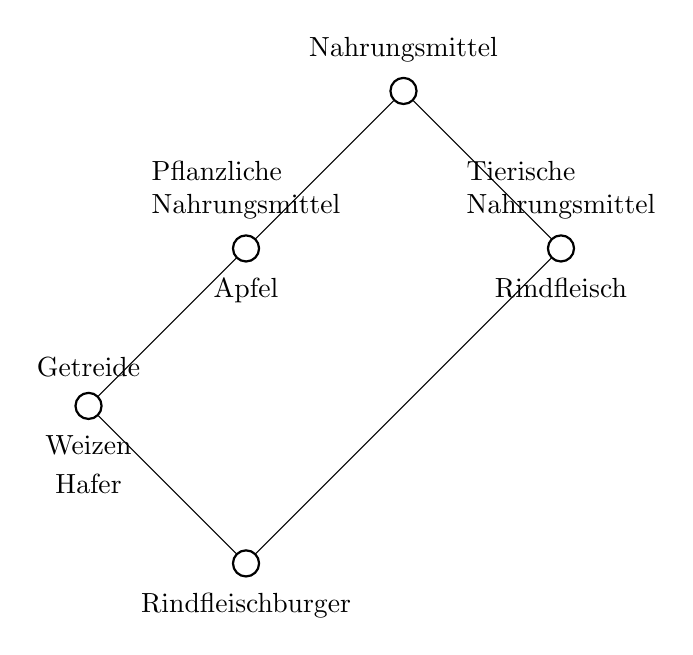
\begin{tikzpicture}
        \begin{scope}[every node/.style={circle,thick,draw}]
            \node (A) at (4,6) {};
            \node (B) at (2,4) {};
            \node (C) at (6,4) {};
            \node (D) at (0,2) {};
            \node (E) at (2,0) {};
        \end{scope}

        % Merkmale
        \draw (A) +(0,0.25) node[above] {Nahrungsmittel};
        \draw (B) +(0,0.25) node[above, align=left] {Pflanzliche\\ Nahrungsmittel};
        \draw (C) +(0,0.25) node[above, align=left] {Tierische\\ Nahrungsmittel};
        \draw (D) +(0,0.25) node[above] {Getreide};

        % Gegenstände
        \draw (B) +(0,-0.25) node[below] {Apfel};
        \draw (C) +(0,-0.25) node[below] {Rindfleisch};
        \draw (D) +(0,-0.25) node[below] {Weizen};
        \draw (D) +(0,-0.75) node[below] {Hafer};
        \draw (E) +(0,-0.25) node[below] {Rindfleischburger};

        % Relationen
        \draw (A) -- (B);
        \draw (A) -- (C);
        \draw (B) -- (D);
        \draw (C) -- (E);
        \draw (D) -- (E);
    \end{tikzpicture}
    \caption{\label{fig:begriffsverband}Begriffsverband - Nahrungsmittel}
\end{figure}

Die Daten aus \autoref{table:fca-food} können als ein Begriffsverband dargestellt werden.
Dieser ist in \autoref{fig:begriffsverband} dargestellt und ist analog zu einem Hasse-Diagramm aufgebaut.
Ein einzelner Knoten repräsentiert einen formalen Begriff.
Dabei stehen die Knoten in einer hierarchischen Relation zueinander.
Über dem Knoten werden die Merkmale und unter dem Knoten die Gegenstände aufgeführt.
Im gegebenem Beispiel ist der Gegenstand Apfel unter dem Merkmal pflanzliche Nahrungsmittel zu finden.
Da dieser Knoten unterhalb des Knotens Nahrungsmittel liegt, ist der Gegenstand Apfel ebenfalls ein Nahrungsmittel.
Es existieren zusätzlich Knoten, welche keine Merkmale besitzen, sondern nur Gegenstände.
In diesem Beispiel ist dies der Knoten mit dem Gegenstand Rindfleischburger.
Das Merkmal dieses Knoten ist implizit durch die Merkmale der übergeordneten Knoten gegeben. \\

\colorlet{mivertexcolor}{blue}
\colorlet{jivertexcolor}{red}
\colorlet{vertexcolor}{mivertexcolor!50}
\colorlet{bordercolor}{black!80}
\colorlet{linecolor}{gray}
% parameter corresponds to the used valuation function and can be addressed by #1
\tikzset{vertexbase/.style 2 args={semithick, shape=circle, inner sep=2pt, outer sep=0pt, draw=bordercolor},%
    vertex/.style 2 args={vertexbase={#1}{}, fill=vertexcolor!45},%
    mivertex/.style 2 args={vertexbase={#1}{}, fill=mivertexcolor!45},%
    jivertex/.style 2 args={vertexbase={#1}{}, fill=jivertexcolor!45},%
    divertex/.style 2 args={vertexbase={#1}{}, top color=mivertexcolor!45, bottom color=jivertexcolor!45},%
    conn/.style={-, thick, color=linecolor}%
}
\begin{figure}
    \centering
    \begin{adjustbox}{max width=\textwidth}
        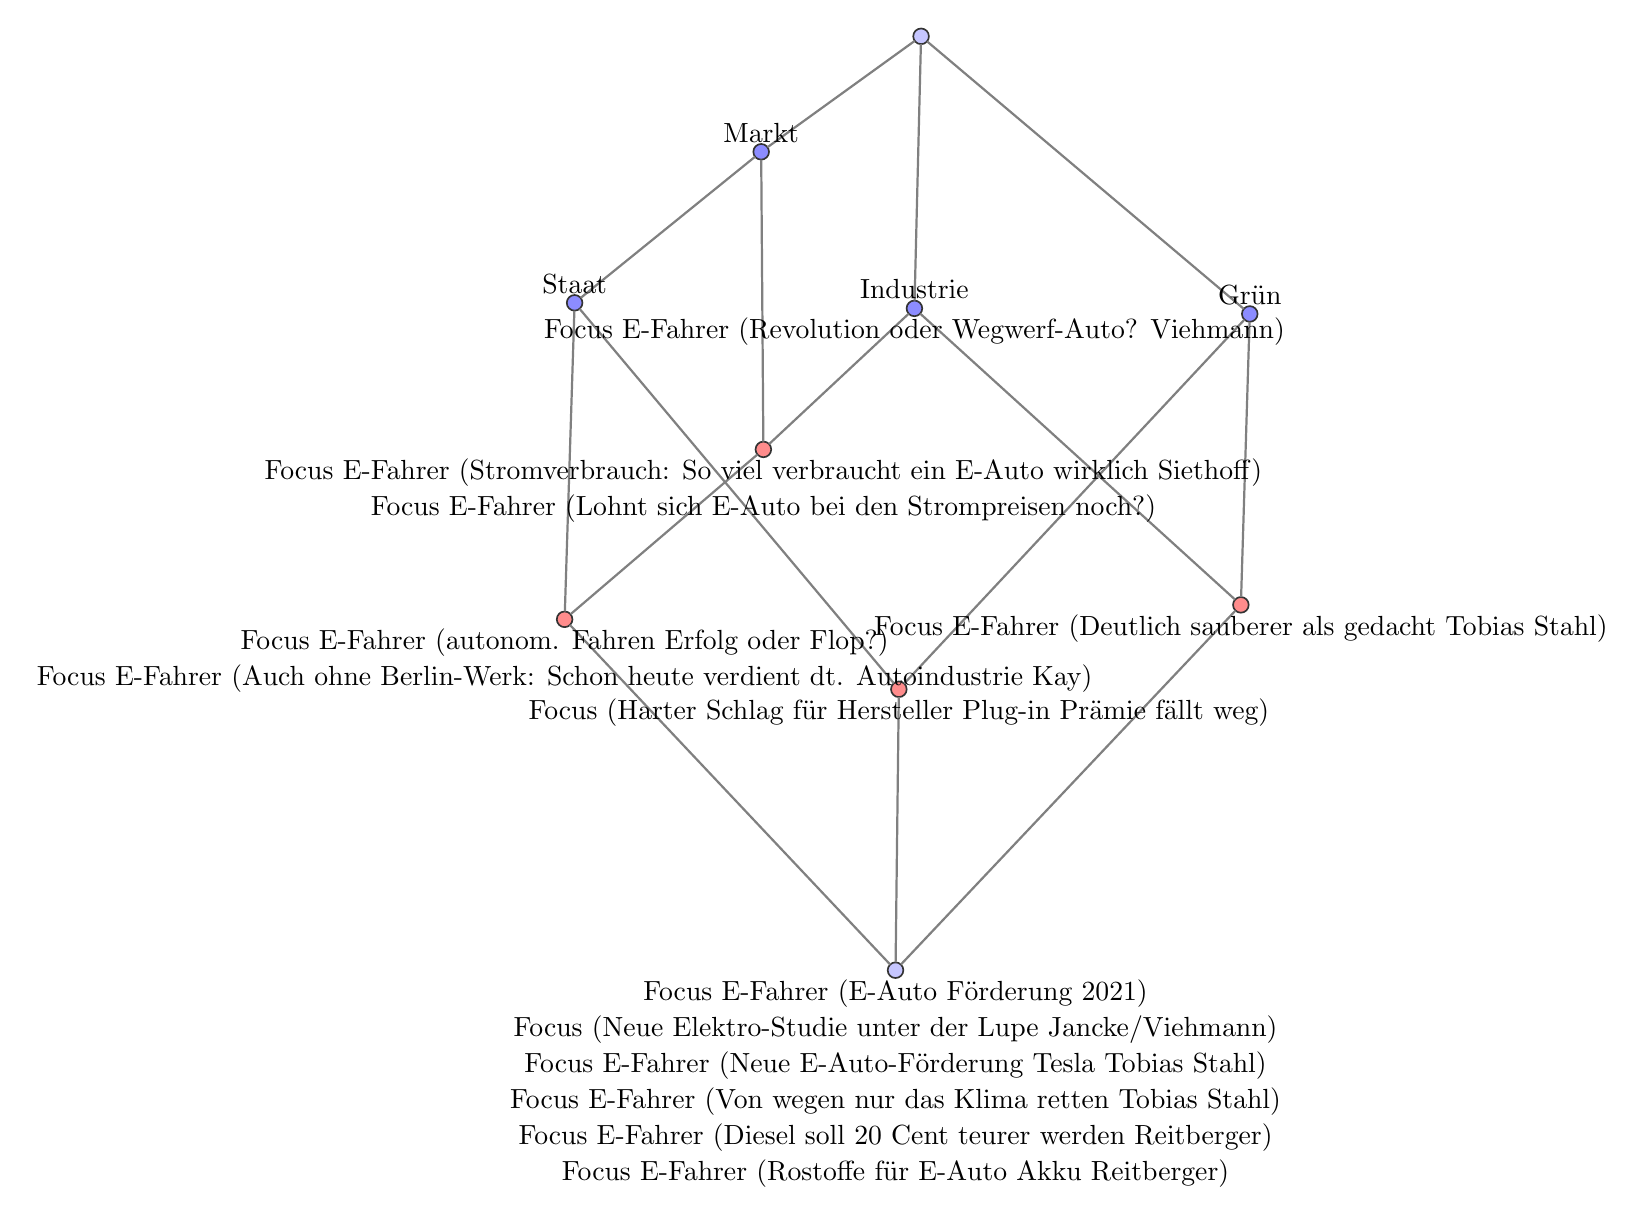
\begin{tikzpicture}
            \begin{scope} %for scaling and the like
                \begin{scope} %draw vertices
                    \foreach \nodename/\nodetype/\param/\xpos/\ypos in {%
                            0/vertex//-0.9525641025641018/2.73846153846155,
                            1/jivertex//-0.9102564102564106/6.306410256410267,
                            2/jivertex//-5.155128205128204/7.194871794871805,
                            3/jivertex//3.4333333333333336/7.378205128205138,
                            4/jivertex//-2.6307692307692303/9.352564102564113,
                            5/mivertex//3.546153846153846/11.073076923076933,
                            6/mivertex//-0.7128205128205121/11.143589743589754,
                            7/mivertex//-5.028205128205128/11.214102564102575,
                            8/mivertex//-2.6589743589743584/13.132051282051293,
                            9/vertex//-0.6282051282051277/14.598717948717958
                        } \node[\nodetype={\param}{}] (\nodename) at (\xpos, \ypos) {};
                \end{scope}
                \begin{scope} %draw connections
                    \path (8) edge[conn] (9);
                    \path (3) edge[conn] (5);
                    \path (3) edge[conn] (6);
                    \path (5) edge[conn] (9);
                    \path (0) edge[conn] (3);
                    \path (0) edge[conn] (1);
                    \path (0) edge[conn] (2);
                    \path (1) edge[conn] (5);
                    \path (1) edge[conn] (7);
                    \path (2) edge[conn] (4);
                    \path (2) edge[conn] (7);
                    \path (4) edge[conn] (8);
                    \path (4) edge[conn] (6);
                    \path (7) edge[conn] (8);
                    \path (6) edge[conn] (9);
                \end{scope}
                \begin{scope} %add labels
                    \foreach \nodename/\labelpos/\labelopts/\labelcontent in {%
                    5/above//{Grün},
                    6/above//{Industrie},
                    7/above//{Staat},
                    8/above//{Markt},
                    0/below//{\shortstack{Focus E-Fahrer (E-Auto Förderung 2021) \\ Focus (Neue Elektro-Studie unter der Lupe Jancke/Viehmann) \\ Focus E-Fahrer (Neue E-Auto-Förderung Tesla Tobias Stahl) \\ Focus E-Fahrer (Von wegen nur das Klima retten Tobias Stahl) \\ Focus E-Fahrer (Diesel soll 20 Cent teurer werden Reitberger) \\ Focus E-Fahrer (Rostoffe für E-Auto Akku Reitberger)}},
                    1/below//{Focus (Harter Schlag für Hersteller Plug-in Prämie fällt weg)},
                    2/below//{\shortstack{Focus E-Fahrer (autonom. Fahren Erfolg oder Flop?) \\ Focus E-Fahrer (Auch ohne Berlin-Werk: Schon heute verdient dt. Autoindustrie Kay)}},
                    3/below//{Focus E-Fahrer (Deutlich sauberer als gedacht Tobias Stahl)},
                    4/below//{\shortstack{Focus E-Fahrer (Stromverbrauch: So viel verbraucht ein E-Auto wirklich Siethoff) \\ Focus E-Fahrer (Lohnt sich E-Auto bei den Strompreisen noch?)}},
                    6/below//{Focus E-Fahrer (Revolution oder Wegwerf-Auto? Viehmann)}
                    } \coordinate[label={[\labelopts]\labelpos:{\labelcontent}}](c) at (\nodename);
                \end{scope}
            \end{scope}
        \end{tikzpicture}
    \end{adjustbox}
    \caption{\label{fig:fba-artikel}Begriffsverband - Artikel}
\end{figure}
